%*******************************************************************************
%****************************** Second Chapter *********************************
%*******************************************************************************

\chapter{Event Detection Using Sum-max Feature Aggregation}
\label{chapter4}
\epigraph{\textit{A clay pot sitting in the sun will always be a clay pot. It has to go through the white heat of the furnace to become porcelain.}}{ -- Mildred W. Struven}

\ifpdf
    \graphicspath{{Chapter4/Figs/Raster/}{Chapter4/Figs/PDF/}{Chapter4/Figs/}}
\else
    \graphicspath{{Chapter4/Figs/Vector/}{Chapter4/Figs/}}
\fi

\section{Introduction}
\label{sec:intro}

The problem of aggregating low level representation into a higher level one has been well studied for image representation. Basically there are two main strategies to aggregate local image descriptors: sum pooling \cite{Koenderink:1999} and max pooling \cite{Serre05objectrecognition}. To understand about these pooling strategies, it is better to mention them in the context of bag-of-word model \cite{Csurka04visualcategorization}. In this model, at first a dictionary or codebook with around thousands of codewords is trained using an unsupervised method such as K-means or Approximate K-means. After that, local features, which are often extracted using a standard SIFT \cite{Lowe:2004} feature, are quantized into the codebook based on their distances to the nearest codewords. Finally, features that are assigned to a codeword are pooled to get a representative value for that codeword. The sum pooling technique simply takes a sum over responses to a visual word. This technique is useful when most of the features are relevant. On the other hand, the max pooling technique only select the largest value between features responding to a visual word. This technique only useful when at least one local feature is sufficiently discriminative. In this case, most of the remaining features can be irrelevant. \index{k-means}

\index{sum pooling} \index{max pooling} 
Sum pooling and max pooling techniques can be easily adopted for video representation. In this case, we can treat spatial-temporal local features in video as local features in image and apply the same framework. State of art performance can be obtained using bag-of-words model with the sum pooling technique in simple video classification/recognition tasks such as sports action videos \cite{Rodriguez2008} or studio setting movies \cite{marszalek09}. This is due to the fact that discriminative features exist in the entire video in these datasets. However, this observation is not true on complex video datasets where the discriminative features may exist within a small part of the video. One example of these datasets is the TRECVID Multimedia Event Detection (MED) dataset\footnote{http://www.nist.gov/itl/iad/mig/med10.cfm}, where most videos are captured by internet users and it tends to be noisy. Example of such noisy video is shown in Fig \ref{f_teaser}. In this case, video pooling for event recognition is much more challenging.
\begin{figure}
	\centering
	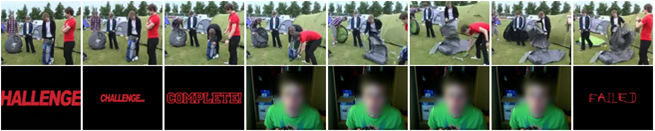
\includegraphics[width=1\textwidth]{teaser_image.png}
	\caption{Example video for "assembling a shelter" event in the TRECVID MED 2010 dataset. The top row shows the relevant frames while the bottom row shows the noisy frames.}
	\label{f_teaser}
\end{figure}

We are interested in the problem of video pooling for a more robust video representation. We consider a video as a layered structure where the lowest layer are frames, the top layer is the entire video, and the middle layers are the sequences of consecutive frames or the concatenation of lower layers. Based on this layered structure of video, we propose to use the sum-max video pooling to deal with noisy information in complex videos. Basically, we apply sum pooling at the low layer representation while using max pooling at the high layer representation. Sum pooling is used to keep sufficient relevant features at the low layer, while max pooling is used to retrieve the most relevant features at the high layer, therefore it can discard irrelevant features in the final video representation. \index{video representation}

Our work is most related to \cite{DBLP:journals/vlsisp/PhanNLTLDS14}, in which they proposed a segment-based approach to generate segment level representation using the sum pooling technique. Here we focus on different pooling techniques to generate the video representation. Experimental results on the TRECVID Multimedia Event Detection 2010 dataset shows the effectiveness of our method.

The rest of this chapter is organized as follows. Section 2 introduces the layered structure of video. Section 3 presents our sum-max pooling technique based on this layered structure. The experimental setup and experimental results are described in Section 4. Finally, Section 5 concludes this chapter with discussions on our future work.

\section{Layered Structure of Video} \index{layer structure}
\label{sec:format}
As mentioned in the previous section, pooling over the whole video is not effective for complex video representation because these videos can contain irrelevant information. The direct solution to remove these irrelevant information from the final video representation is to pool over the relevant parts only. However, it is also non-trivial to determine which parts of the video are relevant or not. 
\begin{figure}[!htb]
	\centering
	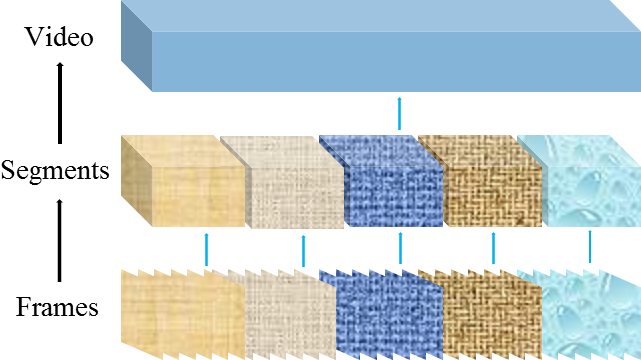
\includegraphics[width=1\textwidth]{layered.png}
	\caption{Illustration of layered structure of video.}
	\label{f_layer}
\end{figure}

The layered structure of video is a simply way to lessen the impact of irrelevant information. We define this layered structure as follows. The lowest layer are the frames of that video. The top layer is the entire video. The middle layers are the sequences of consecutive frames or the concatenation of lower layers. Figure \ref{f_layer} illustrates the layered structure in videos.

For the sake of simplicity, we only use one middle layer and the frame sequences in the middle layer are referred as segments in the rest of this chapter. In implementation, we choose the length of the segments varies in the following range: 15, 30, 45, 60, 75, 90, 105, 120, 135, 150, 165, 180, 195 and 210 seconds. We report the best segment length in Section \ref{c4_experiment}.

\section{Sum-max Video Pooling} \index{sum-max video pooling}
\label{sec:summax}
\begin{figure}
	\centering
	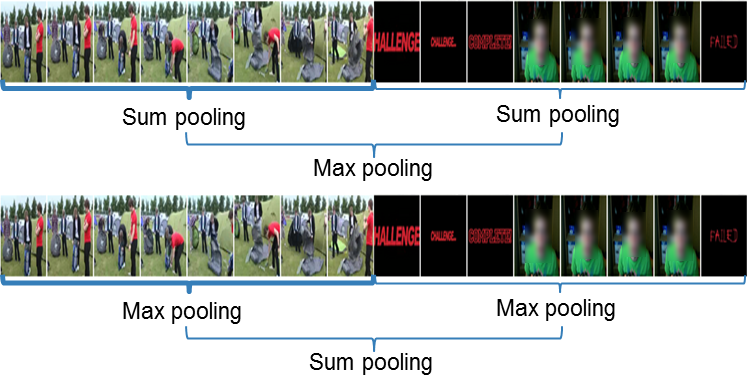
\includegraphics[width=1\textwidth]{summax_maxsum.png}
	\caption{Example of applying sum-max video pooling (top) and max-sum video pooling (bottom) methods on an ``assembling a shelter'' event video. It can be seen from the top image that after applying max pooling at the segment level, only relevant frames are encoded in the final representation.}
	\label{f_sum_max3}
\end{figure}

\begin{figure}
	\centering
	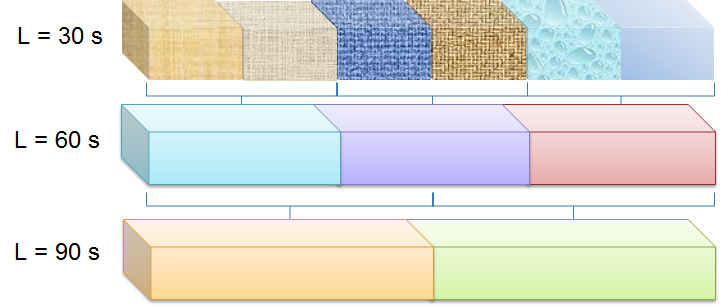
\includegraphics[width=1\textwidth]{efficient.png}
	\caption{Features from higher layers can be obtained from lower layers efficiently.}
	\label{f_efficient}
\end{figure}

\begin{figure}[!htb]
	\centering
	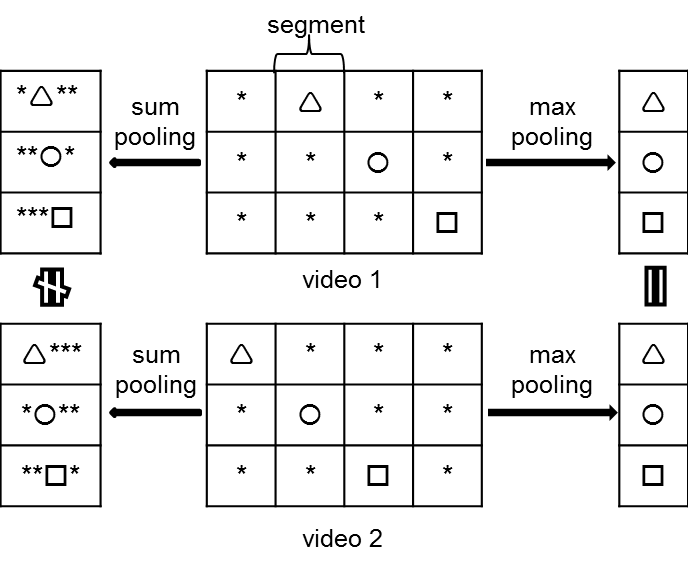
\includegraphics[width=1\textwidth]{sum_max.png}
	\caption{Illustration of sum-max video pooling. $\triangle$, O, $\Box$ represent relevant information; * represents different kinds of irrelevant information, which is popular in complex event data. Due to the native of the data, relevant information can appear in any part of the video, and can follow some temporal order. }
	\label{f_sum_max}
\end{figure}
\begin{figure*}[!htb]
	\centering
	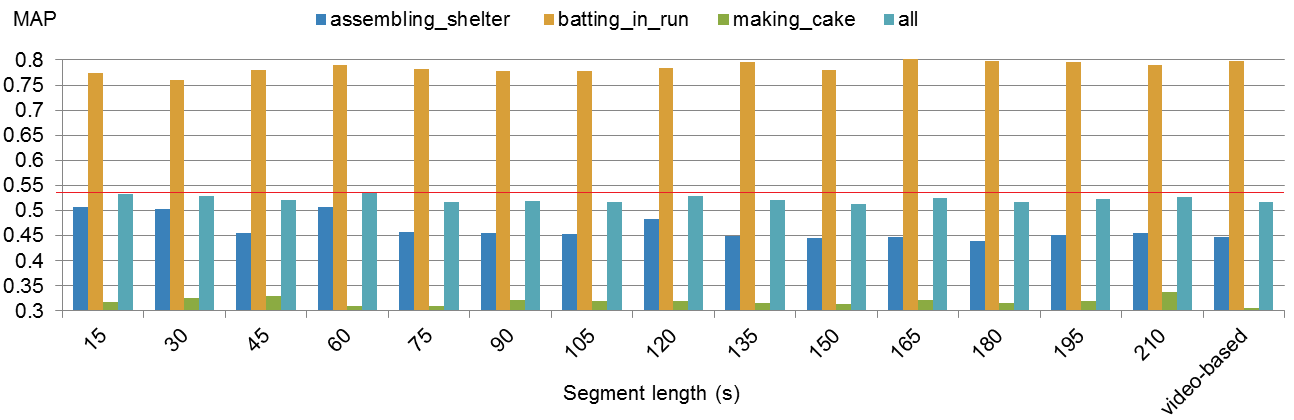
\includegraphics[width=1\textwidth]{sum_max_chart.png}
	\caption{Results on the MED 2010 dataset using the sum-max pooling technique at different segment lengths.}
	\label{f_sum_max_chart}
\end{figure*}
\begin{figure*}[!htb]
	\centering
	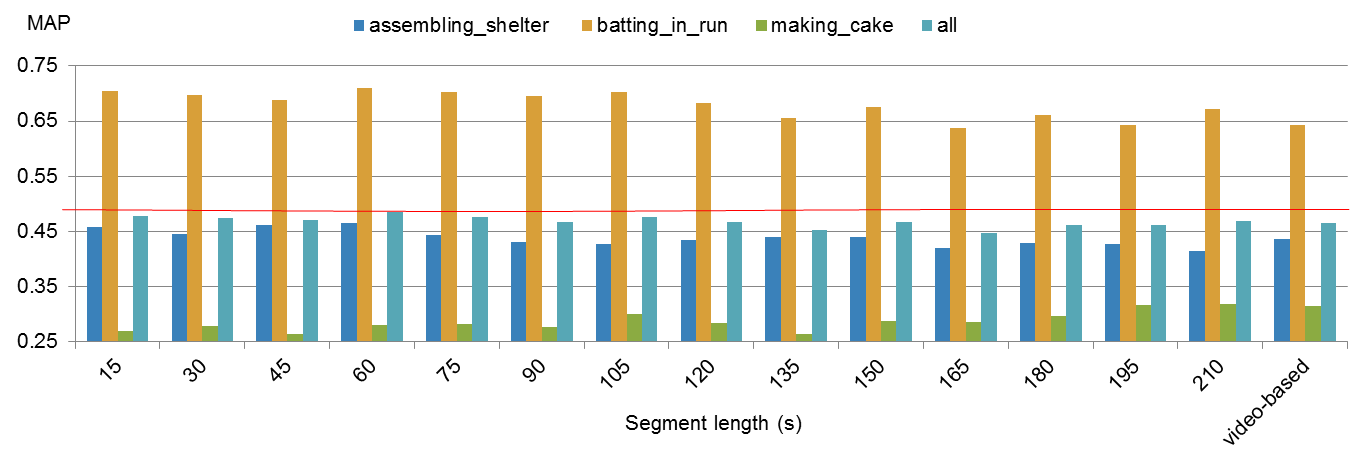
\includegraphics[width=1\textwidth]{max_sum_chart.png}
	\caption{Results on the MED 2010 dataset using the max-sum pooling technique at different segment lengths.}
	\label{f_max_sum_chart}
\end{figure*}
Our sum-max video pooling method is proposed based on the layered structure of video and consists of two steps: (1) Applying sum pooling to aggregate features from all frames of each segment to generate the feature representation of that segment; (2) Applying max pooling to aggregate the segment-level features to form the video representation. The max-sum video pooling can be obtained in the same way but different in that max pooling is applied first, then the sum pooling. It is worth noted that, sum video pooling and max video pooling are two special cases when we applying sum-max video pooling and max-sum video pooling for the whole video respectively. Examples of sum-max and max-sum video pooling are shown in Fig \ref{f_sum_max3}. 

In the context of bag-of-words model, suppose that there are N local descriptors in the video, each descriptor is denoted at $x_{n} \in R^{D}$, where n = 1,...,N and D is the feature dimension. Denote each visual word $m_{k} \in R^{D}$, where k = 1,...,K with K is number of visual words. $M = \{m_{k}\}$ is the set of visual words. The mid level coding of each descriptor can be expressed as $\phi_{n} = [\Phi_{1n},...,\Phi_{Kn}]$. Further suppose that the video contains \textit{S} segments. Denote $N_{s}$ is the number of local descriptors in segment \textit{s}. The sum-max and max-sum video pooling at each visual word can be defined as follows:
\begin{equation}\psi_{k} = Max_{s \in S}(\sum_{n \in N_{s}}\Phi_{kn})\end{equation}

\begin{equation}\psi_{k} = \sum_{s \in S}(Max_{n \in N_{s}}\Phi_{kn})\end{equation}

An intuitive example of sum-max pooling is shown in Fig \ref{f_sum_max}. As we can see, max pooling reserves the relevant information because noisy data tend to be varied, and none of any kind of them is dominant. In the contrast, sum pooling incorporates both relevant and irrelevant ones. Therefore, it is less representative than max pooling.

It is also worth noted that features from higher layers can be obtained from lower layers efficiently. In fact, we only need to extract feature one time. An illustration of features calculated from different segment lengths can be seen on Fig. \ref{f_efficient}.

\section{Experiment}
\label{c4_experiment}
\subsection{Experimental Setup}
We tested our method on TRECVID MED 2010 dataset. An event kit is provided with the definitions and textual descriptions for all the events for each dataset. The first dataset contains 3,468 videos, including 1,744 videos for training and 1,724 video clips for testing, containing a total of more than 110 video hours. In TRECVID MED 2010, there are 3 event classes: \textit{assembling a shelter} (E001), \textit{batting in a run} (E002), and \textit{making a cake} (E003).

We adopt the popular bag-of-words model to build our event recognition framework. At first, we use dense trajectory motion feature published by Wang \cite{wang:2011:inria-00583818:1} to calculate raw motion features as local trajectory descriptors. The library to extract these features is published online by the author\footnote{http://lear.inrialpes.fr/people/wang/dense\_trajectories}. The source code is customized for pipeline processing using only Motion Boundary Histogram (MBH) descriptor to save computing time but other parameters are set to default. 

In the coding step, we randomly select 1,000,000 dense trajectories for clustering to form a codebook of 4000 visual codewords. After that, the frequency histogram of the visual words is computed over each segment to generate the feature vector for that segment. Finally, we apply the sum-max pooling technique as described in Section \ref{sec:summax} to obtain the final video representation. We also adopt the soft assignment weighting scheme \cite{Jiang:2007:TOB} with 5 nearest neighbors to improve the performance of the ``bag-of-words'' approach.

In the learning and testing step, we use the popular Support Vector Machine (SVM) for event classification. In particular, we use the LibSVM library available online\footnote{http://www.csie.ntu.edu.tw/{\textasciitilde}cjlin/libsvm/} and adopt the one-vs.-rest scheme for multi-class classification. 

\subsection{Experimental Result and Analysis}

\subsubsection{On the MED 2010 dataset}
We report the results in terms of the Mean Average Precision (MAP). Results of sum-max video pooling and max-sum video pooling are showed in Fig \ref{f_sum_max_chart} and Fig \ref{f_max_sum_chart} respectively. Sum-max pooling improves the overall performance, especially for ``assembling a shelter'' event. The best performance is obtained at the segment length of 60 s (same as observed in \cite{DBLP:journals/vlsisp/PhanNLTLDS14}). Max-sum video pooling did not achieve good results compared to sum-max video pooling. The reason for the low performance of max-sum pooling can be due to the lost of relevant information when max-pooling is applied first. 

We also observed that the performance largely depends on the segment length and the event itself. For example, we can get better performance with short segment lengths for the event ``assembling a shelter'', while the event ``making a cake'' tends to have better performance with longer segments. 

We summarize our experimental results in Table \ref{t_med10}. The best performing feature is highlighted in bold for each event. In general, pooling over segments is more effective, i.e, sum-max pooling outperforms sum pooling and max-sum pooling outperforms max pooling. In the best case, sum-max video pooling outperforms the traditional sum pooling up to 2\% in terms of MAP.

\begin{table}
	\renewcommand{\arraystretch}{1.3}
	\caption{Performance comparison of different video pooling strategies on the MED 2010 dataset.}
	\label{t_med10}
	\centering
	\begin{tabular}{|c|c|c|c|c|}
		\toprule
		Event/MAP & \begin{tabular}[x]{@{}c@{}}Max\\pooling \end{tabular} & \begin{tabular}[x]{@{}c@{}}Sum\\pooling \end{tabular} & \begin{tabular}[x]{@{}c@{}}Max-sum\\pooling\\(at 60 s)\end{tabular} & \begin{tabular}[x]{@{}c@{}}Sum-max\\pooling\\(at 60 s)\end{tabular} \\
		%\bfseries \begin{tabular}[c]{@{}c@{}} CU\\(SIFT)\end{tabular}&
		%\bfseries \begin{tabular}[c]{@{}c@{}}CU (STIP,\\SIFT,\\MFCC)\end{tabular}\\
		\midrule
		E001&0.4365&0.4468&0.4646&\textbf{0.5072}
		\\
		\midrule
		E002&0.6434&\textbf{0.7988}&0.7103&0.7900
		\\
		\midrule
		E003&\textbf{0.3144}&0.3053&0.2806&0.3100
		\\
		\midrule
		All&0.4648&0.5170&0.4852&\textbf{0.5357}
		%&0.512&0.633
		\\
		\bottomrule
	\end{tabular}
\end{table}

\subsubsection{On the MED 2011 dataset}

In this experiment, we calculate the sum-max video pooling at different segment lengths including 8 s, 16 s, 32 s, 64 s, 128 s and 256 s. Results of our proposed methods on MED 2011 dataset are shown on Fig. \ref{f_med11_summax_kernel} and Fig. \ref{f_med11_summax_linear} respectively. Our best results are obtained at 8 s when using ${\chi}^2$ SVM and 32 s when using linear SVM.

\begin{figure*}[!htb]
	\centering
	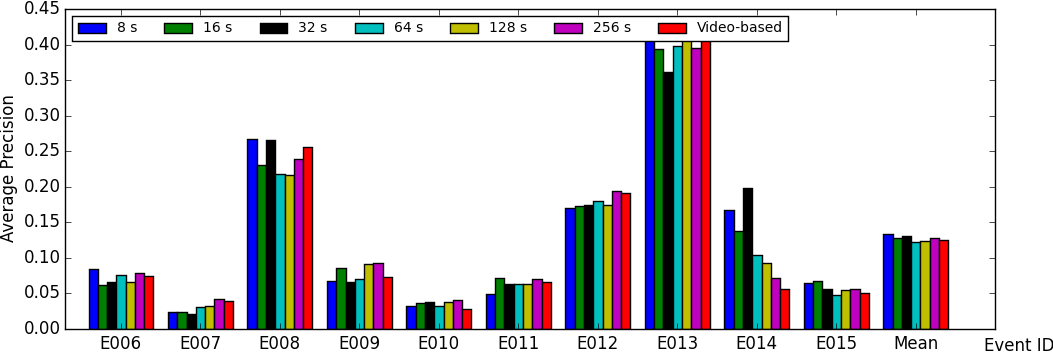
\includegraphics[width=1\textwidth]{med11_summax_kernel.png}
	\caption{Results on the MED 2011 dataset using the sum-max pooling technique at different segment lengths (${\chi}^2$ SVM).}
	\label{f_med11_summax_kernel}
\end{figure*}

\begin{figure*}[!htb]
	\centering
	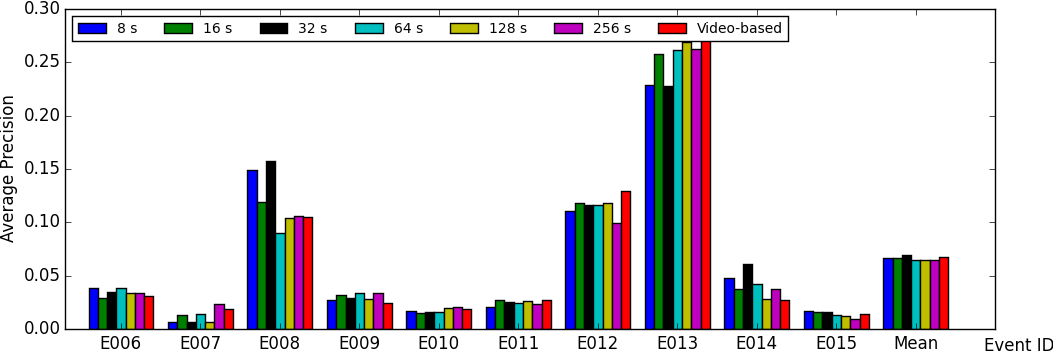
\includegraphics[width=1\textwidth]{med11_summax_linear.png}
	\caption{Results on the MED 2011 dataset using the sum-max pooling technique at different segment lengths (linear SVM).}
	\label{f_med11_summax_linear}
\end{figure*}


\section{Conclusion}
\label{sec:majhead}

We proposed to use a sum-max video pooling technique to combine both sum pooling and max pooling into a holistic video representation. This pooling technique is based on the layered structure of video. Preliminary results showed that this is an promising direction for video representation.

One limitation of the current approach is that the performance depends on the segment length. Therefore, we suggest to investigate a better approach to utilize the layered structure of video for video representation.

For video representation, temporal information is also very important. However, it is difficult to encode temporal information because video lengths are very varied. Therefore, exploring temporal pooling for video representation is also a good research direction.  

